\documentclass[11pt]{beamer}
\usetheme{Boadilla}
\usecolortheme{seahorse}
\usepackage[utf8]{inputenc}
\usepackage[spanish]{babel}
\usepackage{amsmath}
\usepackage{amsfonts}
\usepackage{amssymb}
\usepackage{graphicx}
\usepackage{algorithm}
\usepackage[]{algpseudocode}
\usepackage{varwidth}
\usepackage{float}

\usepackage{movie15}
\usepackage{hyperref}

\floatname{algorithm}{Algoritmo}
\algrenewcommand\algorithmicrequire{\textbf{Requiere}}
\algrenewcommand\algorithmicfor{\textbf{Para}}
\algrenewcommand\algorithmicdo{\textbf{hacer}}
\algrenewcommand\algorithmicif{\textbf{si}}
\algrenewcommand\algorithmicthen{\textbf{entonces}}
\algrenewcommand\algorithmicelse{\textbf{sino}}
\algrenewcommand\algorithmicreturn{\textbf{Retornar}}
\algrenewcommand\algorithmicend{\textbf{Fin}}
\algrenewcommand\algorithmicfunction{\textbf{Función}}
\algrenewcommand\algorithmicprocedure{\textbf{Procedimiento}}
\algrenewcommand\alglinenumber[1]{\tiny #1:}
%\usepackage{lmodern}

\DeclareMathOperator*{\argmin}{argmin}
\DeclareMathOperator*{\argmax}{argmax}

%-----------------------------------------------------------------
%	TITLE PAGE
%-----------------------------------------------------------------

\author[Carolina Higuera Arias]{Carolina Higuera Arias\\ \bigskip \textit{Asesor:} Ph.D Fernando Enrique Lozano Martinez}
\title[Control de tránsito con MARL]{Control de intersecciones semaforizadas aplicando aprendizaje por refuerzo multiagente}
\institute[Uniandes] 
{
Universidad de los Andes \\ 
\medskip
}
\titlegraphic{
\includegraphics[scale=0.5]{./graficas/uniandes.eps}}
\date{Diciembre 16, 2016}

\begin{document}

\newenvironment{rcases}
  {\left.\begin{aligned}}
  {\end{aligned}\right\rbrace}

%----------D1: presentacion ------------------
\begin{frame}
\titlepage 
\end{frame}

\section{Motivación y definición del problema}
%----------D2: motivacion ------------------
\begin{frame}
\frametitle{Motivación y definición del problema}
\center
\begin{tabular}{cc}
\multicolumn{2}{c}{\textbf{Congestión vehicular en Bogotá}} \\ & \\
Causas & Consecuencias \\ 
\hline  \hline
\begin{minipage}[t]{0.5\textwidth}
\begin{itemize}
 \item Incremento del parque automotor
 \item Atraso en la infraestructura vial
 %\item Mal estado de la malla vial
 \item Semáforos mal programados 
 \end{itemize} 
 \end{minipage}
& 
\begin{minipage}[t]{0.4\textwidth}
 \begin{itemize}
 \item Altos tiempos de espera
 \item Problemas económicos
 \item Problemas ambientales
 \end{itemize} 
 \end{minipage}
\\ 
\end{tabular} 
\bigskip \bigskip
\begin{block}{Pregunta de investigación}
¿Cómo mejorar la infraestructura actual, de tal manera que se haga un uso inteligente y óptimo de los semáforos de la malla vial?
\end{block}
\end{frame}

\section{Solución propuesta}
%----------D3: solucion propuesta ------------------
\begin{frame}
\frametitle{Solución propuesta}
Obtener una estrategia de control con las siguientes características:
\begin{equation*}
\begin{rcases}
 \parbox{18em}{\begin{itemize}
 \item Accionado por el tránsito
 \item Independiente del modelo matemático del sistema
 \item Que busque minimizar objetivos específicos para el sistema
 \end{itemize}}
\end{rcases}
\parbox{10em}{ \begin{center} Aplicar aprendizaje por refuerzo multiagente (MARL) \end{center}}
\end{equation*}

%\begin{table}[]
%\centering
%%\caption{My caption}
%\resizebox{\textwidth}{!}{
%\begin{tabular}{cl|l}
%\multicolumn{1}{l}{} & \multicolumn{1}{c}{\textit{Control por tiempos fijos}} & \multicolumn{1}{c}{\textit{Control adaptativo por MARL}} \\ \cline{2-3} 
%\multicolumn{1}{c|}{Objetivos} & \multicolumn{1}{l|}{} & \multicolumn{1}{l|}{\begin{tabular}[c]{@{}l@{}}Minimizar tiempo de espera y \\ longitud de cola\end{tabular}} \\ \cline{2-3} 
%\multicolumn{1}{c|}{Acciones} & \multicolumn{1}{l|}{\begin{tabular}[c]{@{}l@{}}Fases y tiempos fijos\\ Secuencia cíclica de las fases\end{tabular}} & \multicolumn{1}{l|}{\begin{tabular}[c]{@{}l@{}}Fase y duración de acuerdo al \\ estado del sistema\end{tabular}} \\ \cline{2-3} 
%\end{tabular}}
%\end{table}
\end{frame}

\section{Aprendizaje por refuerzo}
\subsection{RL un agente}
%----------D4: aprendizaje por refuerzo un solo agente ------------------
\begin{frame}
\frametitle{Aprendizaje por refuerzo}
\framesubtitle{Caso de un solo agente:}
\begin{center}
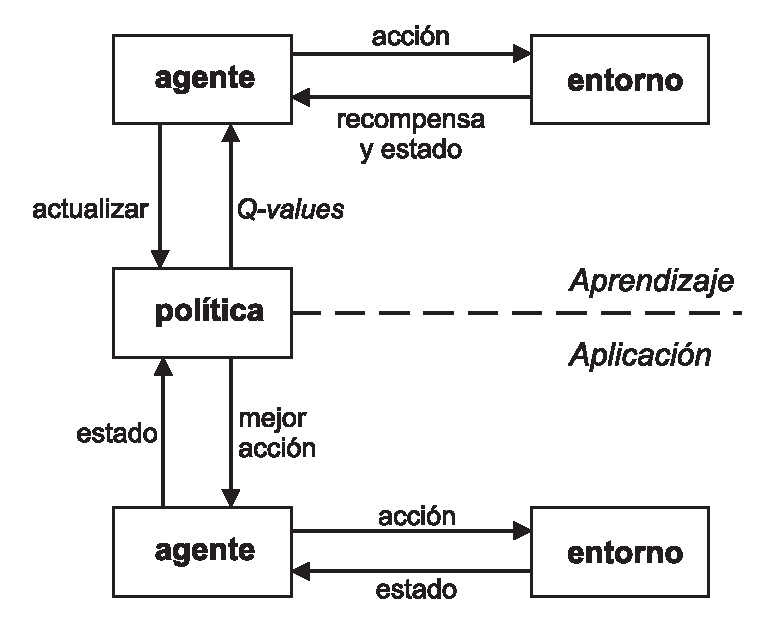
\includegraphics[scale=0.55]{./graficas/singleRL2.eps}
\end{center}
\end{frame}

\subsection{RL multiagente}
%----------D5: aprendizaje por refuerzo multiagente ------------------
\begin{frame}
\frametitle{Aprendizaje por refuerzo}
\framesubtitle{Caso multiagente:}
\centering
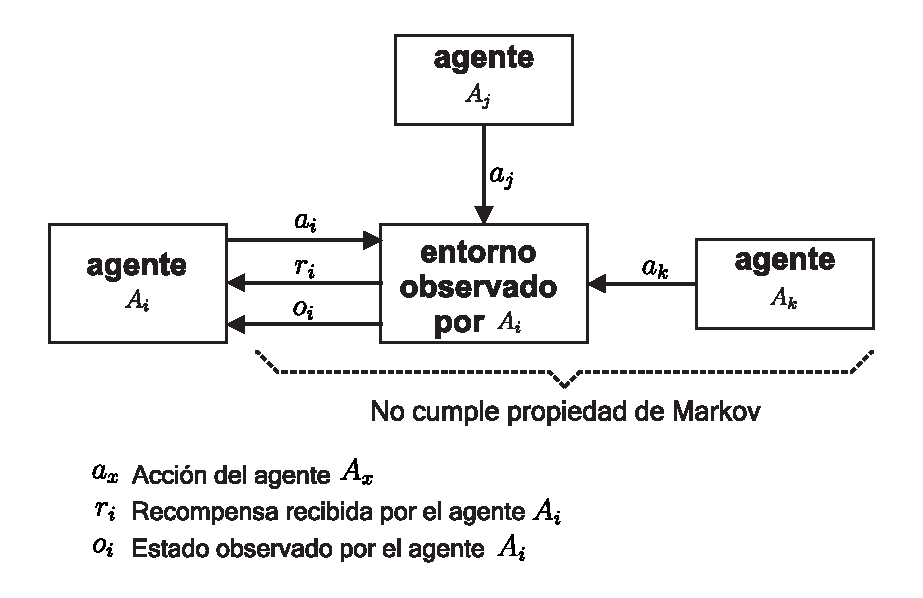
\includegraphics[scale=0.55]{./graficas/multiRL.eps}
\begin{itemize}
\item Se puede describir todo el sistema como un MDP multiagente colaborativo.
\end{itemize}
\end{frame}

%----------D5: aprendizaje por refuerzo multiagente ------------------
\begin{frame}
\frametitle{Aprendizaje por refuerzo}
\framesubtitle{Caso multiagente:}
Sistema multiagente descrito principalmente por:\\
\begin{itemize}
\item Un tiempo discreto $k$
\item Un grupo de $n$ agentes ${A_1, A_2, \cdots, A_n}$
\item Un conjunto finito de estados $\mathbf{s}^k \in \mathcal{S}$
\item Un conjunto de acciones conjuntas $\mathbf{a}^k\in \mathcal{A}$
%\item Un conjunto finito de observaciones del estado $\Omega_i$ para cada agente $i$
%\item Una función de transición de estados $T=\mathcal{S} \times \mathcal{A} \times \mathcal{S}$
\item Una función de recompensa $R_i:\mathcal{S} \times \mathcal{A}\rightarrow \mathbb{R}$ que entrega a cada agente $i$ una recompensa numérica $r_i^k$\\
\end{itemize}
\bigskip
\begin{center}
Donde $\mathbf{R(s^k,a^k)=\sum_{i=1}^{n} R_i(s^k,a^k)}$
\end{center}
\end{frame}

%----------D5: aprendizaje por refuerzo multiagente ------------------
\begin{frame}
\frametitle{Aprendizaje por refuerzo}
\framesubtitle{Caso multiagente:}
Teniendo en cuenta $Q(\mathbf{s},\mathbf{a})=\mathrm{E}\left\lbrace R^k | \mathbf{s}^k=\mathbf{s}, \mathbf{a}^k=\mathbf{a} \right\rbrace $\\
\bigskip
Es posible descomponer la función $Q$ del sistema en una combinación lineal de funciones por agente:
$$Q(\mathbf{s},\mathbf{a})=\sum_{i=1}^{n}Q_i(\mathbf{s}_i,a_i)$$\\
Regla de actualización para el caso multiagente:
$$Q_i^{k+1}(\mathbf{s}_i^k,a_i^k)=(1-\alpha^{k+1})Q_i^k(\mathbf{s}_i^k,a_i^k)+\alpha^{k+1} \left[r_i^{k+1} + \gamma \alert<2>{\max_{\mathbf{a}^\prime \in \mathcal{A}}Q^k(\mathbf{s}^{k+1},\mathbf{a}^\prime)} \right]$$
\pause
\end{frame}

\section{Coordinación en MARL}
%----------D5: coordinacion MARL ------------------
\begin{frame}
\frametitle{Coordinación en MARL}
Emerge la necesidad de coordinación de acciones entre agentes para maximizar la recompensa global a largo plazo\\
\bigskip
\begin{alertblock}{Problema de coordinación}
\begin{center}
Encontrar $\mathbf{a}^\prime = \argmax_{\mathbf{a}^\prime \in \mathcal{A}}Q(\mathbf{s},\mathbf{a}^\prime)$
\end{center}
\end{alertblock}
\end{frame}

%\section{Estado del arte}
%%----------D6: estado del arte ------------------
%\begin{frame}
%\frametitle{Aportes al control de tránsito mediante MARL}
%\framesubtitle{Estado del arte: métodos de coordinación (MC)}
%\begin{center}
%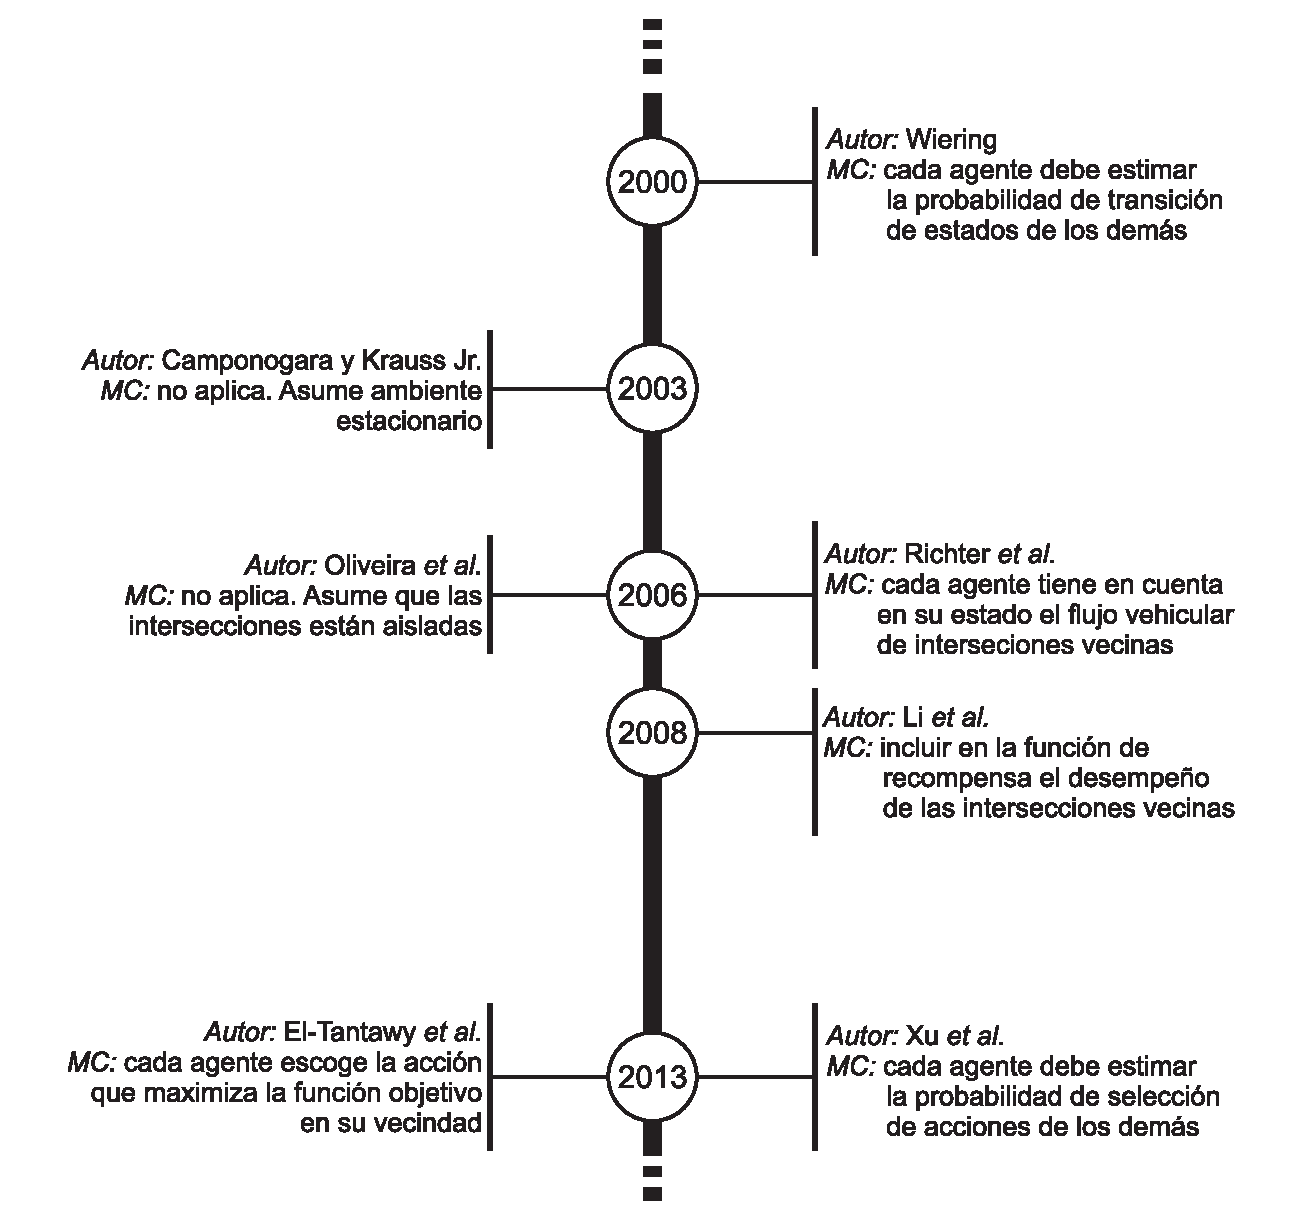
\includegraphics[scale=0.4]{./graficas/estArt2.eps}
%\end{center}
%\end{frame}

\section{Enfoques para establecer coordinación}
%----------D7: enfoques de solucion ------------------
\begin{frame}
\frametitle{Enfoques para establecer coordinación}
\begin{block}{Principio de localidad}
Dos objetos suficientemente alejados uno de otro no pueden influirse mutuamente de manera instantánea.
\end{block}
\bigskip
\textcolor{blue}{En el sistema de tránsito:} la acción de cada agente influye en mayor medida en el estado percibido arededor de su vecindad.\\
\begin{center}
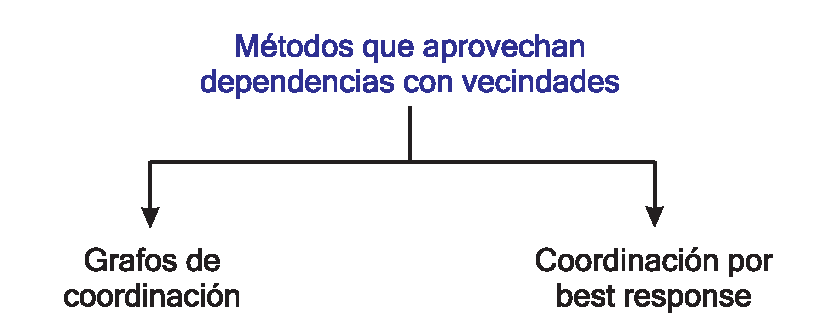
\includegraphics[scale=0.6]{./graficas/solProp.eps}
\end{center}

\end{frame}

\section{Q-Learning y grafos de coordinación}
%----------D8: grafos de coordinacion ------------------
\begin{frame}
\frametitle{Método 1: Q-Learning y grafos de coordinación}
\begin{itemize}
\item Representa, por medio de un grafo $G=(V,E)$, problemas en los cuales el agente $i$ solo exhibe necesidad de coordinación con una vecindad $\Gamma(i)$.\\
\item Permite la descomposición por arco de la función $Q$ global.
\small
\begin{equation*}
Q(\mathbf{s},\mathbf{a})=\sum_{(i,j)\in E}Q_{ij}(\mathbf{s}_{ij},a_i,a_j)
\end{equation*}
\normalsize
\item Regla de actualización con Q-Learning\footnotemark:
\end{itemize}
\small
\begin{equation*}
Q_{ij}^{k+1}(\mathbf{s}_{ij}^k,a_i^k,a_j^k) = (1-\alpha)Q_{ij}^k(\mathbf{s}_{ij}^k,a_i^k,a_j^k) + \alpha\left[ \frac{r_i^{k+1}}{|\Gamma(i)|}+\frac{r_j^{k+1}}{|\Gamma(j)|}+\gamma Q_{ij}^k(\mathbf{s}_{ij}^{k+1},\alert<2>{a_i^*},\alert<2>{a_j^*}) \right]
\end{equation*}
\normalsize
\pause
\bigskip
\small
\begin{equation*}
\alert{a_i^*, a_j^* \in \argmax_{\mathbf{a}^\prime \in \mathcal{A}}Q(\mathbf{s},\mathbf{a}^\prime)}
\end{equation*}
\normalsize
\footnotetext[1]{Propuesto por: J. Kok en \textit{Cooperation and Learning in Cooperative Multiagent Systems.} Ph.D thesis, University of Amsterdam, 2006.}
\end{frame}

\subsection{VE}
%----------D8: grafos de coordinacion VE ------------------
\begin{frame}
\frametitle{Método 1: Q-Learning y grafos de coordinación}
\textcolor{blue}{Algoritmo de eliminación de variable (VE): }resuelve el problema de coordinación, encontrando $\mathbf{a}^*=\argmax_{\mathbf{a}}Q(\mathbf{s},\mathbf{a})$\\
\begin{center}
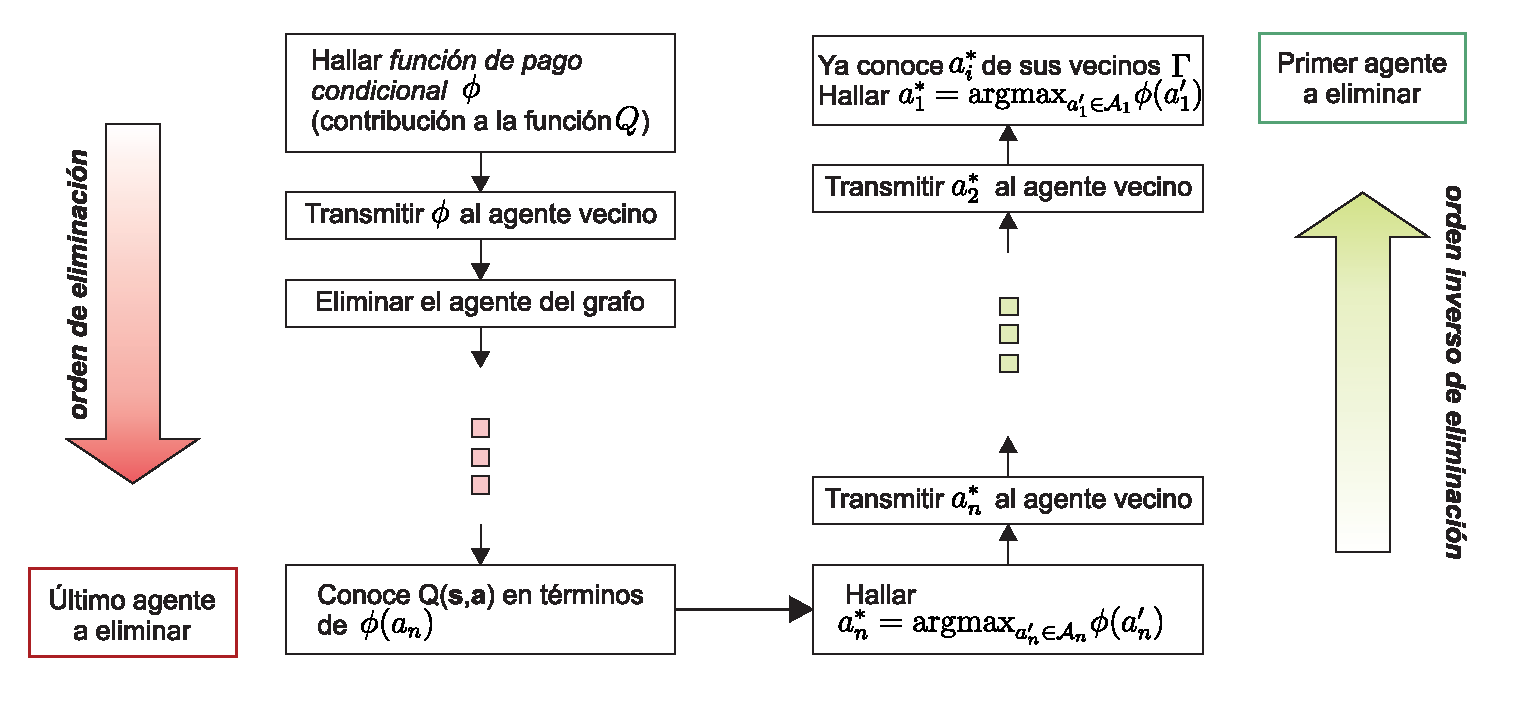
\includegraphics[scale=0.48]{./graficas/ve.eps}
\end{center}
\end{frame}

\subsection{Algoritmo}
%----------D9: grafos de coordinacion: algoritmo ------------------
\begin{frame}[fragile]
\frametitle{Método 1: Q-Learning y grafos de coordinación}
\framesubtitle{Algoritmo de aprendizaje}

\begin{algorithm}[H]
\scriptsize %\small, \footnotesize, \scriptsize, or \tiny
\caption{Q-Learning con eliminación de variable (Q-VE)}\label{alg:Q-VE}
\begin{algorithmic}[]
\State Inicialice $Q_{ij}(s_{ij},a_i,a_j)$ de manera optimista
\For{cada episodio}
	\State Inicialice el estado observado $s_i$ para todos los agentes $i$
	\For{cada periodo de decisión $k$}
		\State Obtenga la acción conjunta $\mathbf{a}$ con $\epsilon-$greedy como método de selección
		\State Para cada agente aplique $a_i \in \mathbf{a}$, observe $r_i^k$ y $s_i^k$
		\State Para todos los arcos $(i,j)$ forme $s_{ij}^k=s_i^k \cup s_j^k$
		\State Obtenga $\mathbf{a}^*=\max_{\mathbf{a}}Q(\mathbf{s^k},\mathbf{a}) \rightarrow$ \Call{EliminaciónVariable}{} 
		\Statex
		\For{cada arco $(i,j)$}
			\State \scriptsize $\begin{aligned}  Q_{ij}(s_{ij}^{k-1},a_i^{k-1},a_j^{k-1}):=& Q_{ij}(s_{ij}^{k-1},a_i^{k-1},a_j^{k-1})+\alpha \left[ \frac{r_i^k}{|\Gamma(i)|}+\frac{r_j^k}{|\Gamma(j)|} + \right. \\ & \left. \gamma Q_{ij}(s_{ij}^k,a_i^*,a_j^*)-Q_{ij}(s_{ij}^{k-1},a_i^{k-1},a_j^{k-1}) {\vphantom{\frac{r_i}{|\Gamma(i)|}}} \right] \end{aligned}$\scriptsize
		\EndFor
		\State Para cada agente $i$ actualice $s_i^{k-1} \leftarrow s_i^k$
	\EndFor
\EndFor
\end{algorithmic}
\end{algorithm}
\end{frame}

\section{Q-Learning y best response}
%----------D10: best response ------------------
\begin{frame}
\frametitle{Método 2: Q-Learning y \textit{best response}}
\begin{columns}[T]
\begin{column}{.6\textwidth}
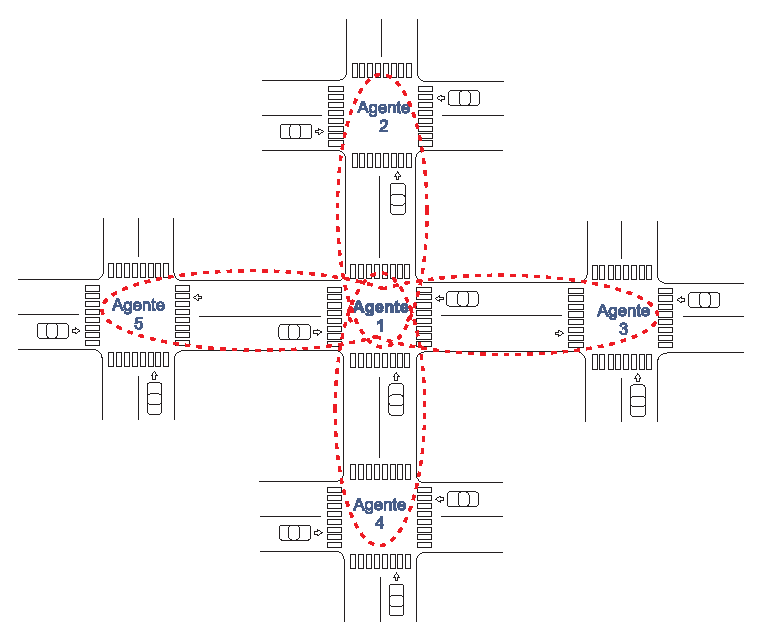
\includegraphics[scale=0.6]{./graficas/exBR.eps}
\end{column}
\begin{column}{.4\textwidth}
El agente $i$:\\
\begin{itemize}
\setlength{\itemindent}{-0.1in}
\item Exhibe necesidad de coordinación con una vecindad $NB_i$
\item Participa en un juego de dos jugadores con cada vecino $NB_i[j]$
%\item Participa en $|NB_i|$ espacios de estados parciales, cuya dimensión siempre será $|\mathcal{S}_i| \times |\mathcal{S}_{NB_i[j]}|$
\end{itemize}
\end{column}
\end{columns}
\end{frame}

\subsection{Pasos}
%----------D10: best response ------------------
\begin{frame}
\frametitle{Método 2: Q-Learning y \textit{best response}}
\only<1>{
El agente $i$ en cada periodo $k$:\\
\medskip
\begin{enumerate}
\item \textcolor{blue}{Estima la política de sus vecinos:}\\
$$\theta_{i,\mathrm{NB}_i[j]}(s_{i,\mathrm{NB}_i[j]}^{k-1}, a_{\mathrm{NB}_i[j]}^{k-1})=\frac{v(s_{i,\mathrm{NB}_i[j]}^{k-1}, a_{\mathrm{NB}_i[j]}^{k-1})}{\sum_{a_{\mathrm{NB}_i[j]} \in \mathcal{A}_{\mathrm{NB}_i[j]}} v(s_{i,\mathrm{NB}_i[j]}^{k-1}, a_{\mathrm{NB}_i[j]})}$$
\end{enumerate}
}
\pause

\only<2,3>{
\bigskip
\begin{enumerate}
\setcounter{enumi}{1}
\item \textcolor{blue}{Actualiza los factores $Q$ con cada vecino:}\\
\end{enumerate}
\footnotesize
$$Q_{i,\mathrm{NB}_i[j]}^{k}(s_{i,\mathrm{NB}_i[j]}^{k-1},a_{i,\mathrm{NB}_i[j]}^{k-1})= (1-\alpha)Q_{i,\mathrm{NB}_i[j]}^{k-1} (s_{i,\mathrm{NB}_i[j]}^{k-1},a_{i,\mathrm{NB}_i[j]}^{k-1}) + \alpha \left[ r_i^k+\gamma \alt<3,4>{\alert<3>{\mathrm{br}_i^k}}{\max_{a^\prime \in \mathcal{A}}Q(s^k,a^\prime)} \right]$$
\normalsize
\visible<3>{
\footnotesize
$$\mathrm{br}_i^k=\max_{a_i \in \mathcal{A}_i} \left[ \sum_{a_{\mathrm{NB}_i[j]} \in \mathcal{A}_{\mathrm{NB}_i[j]}} Q_{i,\mathrm{NB}_i[j]}(s_{i,\mathrm{NB}_i[j]}^k,a_{i,\mathrm{NB}_i[j]}) \times \theta_{i,\mathrm{NB}_i[j]}(s_{i,\mathrm{NB}_i[j]}^k,a_{\mathrm{NB}_i[j]}) {\vphantom{\sum_{a_{NB_i[j]} \in \mathcal{A}_{NB_i[j]}}}} \right]$$ }
\normalsize
%\pause
\only<2,3>{
\visible<3>{
\begin{block}{\textit{Best response}} 
\begin{itemize}
\item Función de pago $Q_i()$
\item Estimativo $\theta_{-i}$ sobre las estrategias de los agentes vecinos
\end{itemize}
La estrategia $a_i \in \mathcal{A}_i$ para el jugador $i$ es una \textit{best response} si para todo ${a_i}^\prime$ se cumple:
$$Q_i(a_i,\theta_{-i}) \geq Q_i({a_i}^\prime,\theta_{-i})$$
\end{block}}}
\pause
}

\only<4>{
\begin{enumerate}
\setcounter{enumi}{2}
\item \textcolor{blue}{Selecciona acción que corresponde a \textit{best response} respecto a su vecindad:}\\
\footnotesize
$$\begin{aligned} a_i^k=\argmax_{a_i \in \mathcal{A}_i}\left[ \sum_{j \in \{1,2,\cdots,|\mathrm{NB}_i|\}} \sum_{a_{\mathrm{NB}_i[j]}\in \mathcal{A}_{\mathrm{NB}_i[j]}} \right. & \left. Q_{i,\mathrm{NB}_i[j]}(s_{i,\mathrm{NB}_i[j]}^k,[a_i \cup a_{\mathrm{NB}_i[j]}]) \right. \times \\ & \left. \theta_{i,\mathrm{NB}_i[j]}(s_{i,\mathrm{NB}_i[j]}^k,a_{\mathrm{NB}_i[j]}) {\vphantom{\sum_{j \in \{1,2,\cdots,|\mathrm{NB}_i|\}}}} \right] \end{aligned}$$
\normalsize
\end{enumerate}
}

\only<4>{
\footnotetext[2]{Basado en: El-Tantawy \textit{et al.} en \textit{Multiagent Reinforcement Learning for MARLIN-ATSC.} IEEE Transactions on Intelligent Transportation Systems, 2013.}
}
\end{frame}

\subsection{Algoritmo}
%----------D10: best response ------------------
\begin{frame}[fragile]
\frametitle{Método 2: Q-Learning y \textit{best response}}
%\framesubtitle{Algoritmo de aprendizaje}

\begin{algorithm}[H]
\scriptsize %\small, \footnotesize, \scriptsize, or \tiny
\caption{Q-Learning con best response (Q-BR)}\label{alg:Q-BR}
\begin{algorithmic}[]
\State Inicialice los factores $Q_{i,NB_i[j]}$ y modelo de estimación de política $\theta_{i,NB_i[j]}$

\For{cada episodio}
	\State Inicialice el estado observado $s_i$ para todos los agentes $i$
	\For{cada periodo de decisión $k$}
		\State Obtenga y aplique la acción conjunta $\mathbf{a}$, con $\epsilon-$greedy como método de selección
%		\State Aplicar $a_i \in \mathbf{a}$ para cada agente $i$
		\For{cada agente $i \in \{1,2,\cdots,|N|\}$}
			\For{cada agente vecino $j \in \{1,2,\cdots,|\mathrm{NB}_i|\}$}
				\State Observe $s_i^k$, $r_i^k$, $s_{\mathrm{NB}_i[j]}^k$ y $a_{\mathrm{NB}_i[j]}^{k-1}$
				\State Forme el estado conjunto $s_{i,\mathrm{NB}_i[j]}^k$ y la acción conjunta $a_{i,\mathrm{NB}_i[j]}^{k-1}$
				\State Actualice el modelo $\theta_{i,\mathrm{NB}_i[j]}(s_{i,\mathrm{NB}_i[j]}^{k-1}, a_{\mathrm{NB}_i[j]}^{k-1})$ de la política

				\State Encuentre la \textit{best response} $br_i^k$

				\State Actualice $Q_{i,\mathrm{NB}_i[j]}^{k}(s_{i,\mathrm{NB}_i[j]}^{k-1},a_{i,\mathrm{NB}_i[j]}^{k-1})$

				\State Actualice $s_{i,\mathrm{NB}_i[j]}^{k-1} \leftarrow s_{i,\mathrm{NB}_i[j]}^k$
			\EndFor

			\State Encuentre al acción $a_i^*$ que corresponde a \textit{best response} con todos los vecinos
		\EndFor
	\EndFor
\EndFor
\end{algorithmic}
\end{algorithm}
\end{frame}

\section{Espacio de estados y acciones}
%----------D11: estados y acciones ------------------
\begin{frame}
\frametitle{Espacio de estados y acciones}
\textcolor{blue}{Vector de estado}\\
Estado de un agente de $i$ accesos ($i \in \{$norte, este, sur, oeste$\}$), conformado por:
\begin{equation*}
\begin{rcases}
\parbox{18em}{\begin{itemize}
\item Hora de día ($h$)
\item Fase actual ($k$)
\item Máxima longitud de cola (veh) por acceso ($q_i$)
\item Tiempo de espera (min) de los vehículos por acceso ($w_i$)
\end{itemize}}
\end{rcases}
\parbox{10em}{\begin{center}
Discretizado por \textit{Vector Quantization}
\end{center} }
\end{equation*}
\medskip

\begin{columns}[T]
\begin{column}{.5\textwidth}
\textcolor{blue}{Acciones}\\
Fase a aplicar con duración mínima:
\begin{itemize}
\item Q-VE: 20 segundos
\item Q-BR: 14 segundos
\end{itemize}
\end{column}
\begin{column}{.5\textwidth}
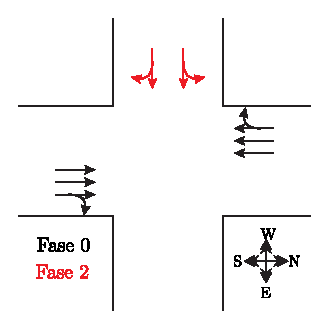
\includegraphics[scale=0.55]{./graficas/ejFases.eps}
\end{column}
\end{columns}
\end{frame}

\section{Función de recompensa}
%----------D11: funcion de recompensa ------------------
\begin{frame}
\frametitle{Función de recompensa para cada agente}
\begin{equation*}\label{eq:rewardQ}
r_i=-\sum_{k=1}^{numAcc_i}\beta_q(q_k)^{\theta_q} + \beta_w(w_k)^{\theta_w}
\end{equation*}
Donde:
\begin{itemize}
\item \textit{$numAcc_i$: } número de accesos que tiene el agente $i$
\item $q_k$: máxima longitud de cola del acceso $k$
\item $w_k$: tiempo de espera de los vehículos en el acceso $k$
\item $\beta_q$ y $\beta_w$: coeficientes para el equilibrio de magnitudes de las variables $q$ y $w$.
\item $\theta_q$ y $\theta_w$: términos potencia para equilibrar las longitudes de cola y tiempos de espera en los accessos.
\end{itemize}
\end{frame}

\section{Marco de prueba}
%----------D12: marco de prueba ------------------
\begin{frame}
\frametitle{Marco de prueba}
\begin{columns}[T]
\begin{column}{.5\textwidth}
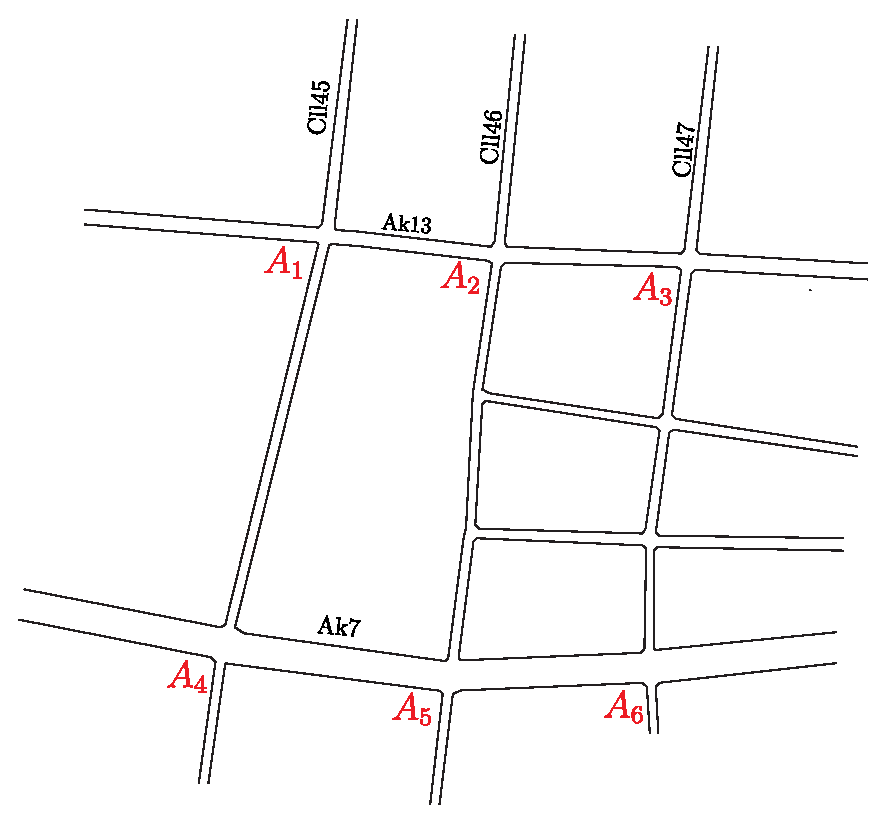
\includegraphics[scale=0.4]{./graficas/minicity.eps}\\
 Datos de flujos vehiculares y programas de fases de la Secretaría de Movilidad de Bogotá
\end{column}
\begin{column}{.5\textwidth}
\textcolor{blue}{Parámetros de simulación:}
\begin{itemize}
\item Interacción con las agentes a través del simulador SUMO
\item \textit{Observación del sistema:} 5 episodios
\item \textit{Aprendizaje de política:} 150 episodios
\item \textit{Prueba de política:} 5 episodios
\end{itemize}
\bigskip
\textcolor{blue}{Detalles de ejecución:}
\begin{itemize}
\item Entrenamiento en AWS
\item Duración: 36 horas aprox.
\end{itemize}
\end{column}
\end{columns}
\end{frame}

\section{Resultados}
\subsection{Curva de aprendizaje}
%----------D13: curva de aprendizaje ------------------
\begin{frame}
\frametitle{Resultados}
\framesubtitle{Curva de aprendizaje}
\begin{columns}[T]
\begin{column}{.47\textwidth}
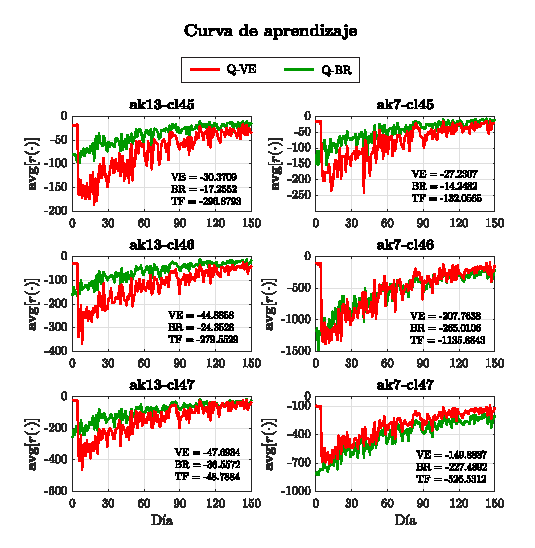
\includegraphics[scale=0.7]{./graficas/rewardEvol.eps}
\end{column}
\begin{column}{.53\textwidth}
\bigskip
\medskip
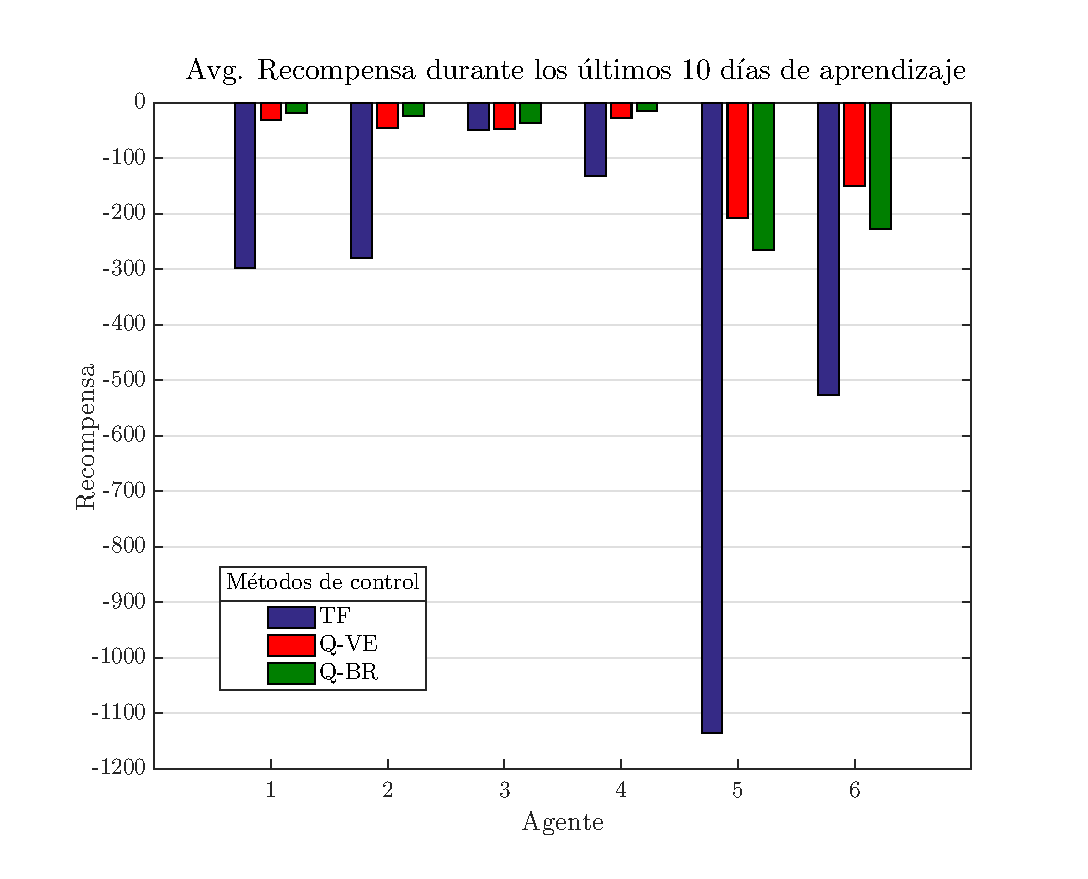
\includegraphics[scale=0.4]{./graficas/lastRew2.eps}
\end{column}
\end{columns}
\end{frame}

\subsection{Indicadores de desempeño}
%----------D13: indicadores de desempeño ------------------
\begin{frame}
\frametitle{Resultados}
\framesubtitle{Indicadores de desempeño}
\begin{itemize}
\item Máxima longitud de cola promedio por intersección (veh)
\item Desviación estándar del promedio de las longitudes de cola en los accesos de las intersecciones (veh)
\item Tiempo de espera promedio por vehículo (s/veh)
\item Velocidad promedio (m/s)
\item  Emisiones promedio de $CO_2$ por intersección (mg)
\end{itemize}

%\begin{table}[]
%\centering
%%\resizebox{\textwidth}{!}{
%\begin{tabular}{l|l}
%\multicolumn{1}{c|}{\textbf{Indicadores primarios}} & \multicolumn{1}{c}{\textbf{Indicadores secundarios}} \\ \hline
%\begin{tabular}[c]{@{}l@{}}\textbullet Máxima longitud de cola promedio\\ por intersección (veh)\end{tabular} & \begin{tabular}[c]{@{}l@{}}\textbullet Desviación estándar del promedio\\ de las longitudes de cola en los \\ accesos de las intersecciones (veh)\end{tabular} \\
%\begin{tabular}[c]{@{}l@{}}\textbullet Tiempo de espera promedio por\\ vehículo (s/veh)\end{tabular} & \textbullet Velocidad promedio (m/s) \\
% & \begin{tabular}[c]{@{}l@{}}\textbullet Emisiones promedio de $CO_2$ \\ por intersección (mg)\end{tabular}
%\end{tabular}
%\end{table}
\end{frame}

\subsection{Indicadores de desempeño del sistema}
%----------D14: indicadores de desempeño del sistema ------------------
\begin{frame}
\frametitle{Resultados}
\framesubtitle{Indicadores de desempeño del sistema}
\begin{table}[]
\resizebox{0.9\textwidth}{!}{
\begin{tabular}{cccccc}
\multicolumn{1}{l}{} & \textit{\begin{tabular}[c]{@{}c@{}}Avg. longitud\\ de cola (veh)\end{tabular}} & \textit{\begin{tabular}[c]{@{}c@{}}Std. Avg. longitud\\ de cola (veh)\end{tabular}} & \textit{\begin{tabular}[c]{@{}c@{}}Avg. tiempo de\\ espera (s/veh)\end{tabular}} & \multicolumn{1}{l}{\textit{\begin{tabular}[c]{@{}l@{}}Avg. velocidad\\ promedio (Km/h)\end{tabular}}} & \multicolumn{1}{l}{\textit{\begin{tabular}[c]{@{}l@{}}Avg. emisiones\\ de $CO_2$ (mg)\end{tabular}}} \\ \hline
\multicolumn{1}{c|}{TF} & 8 & 3 & 38,9 & 15,2 & 5140,9 \\ \hline
\multicolumn{1}{c|}{Q-VE} & 5 & 2 & 16,7 & 15,9 & 4025,8 \\ \hline
\multicolumn{1}{c|}{Q-BR} & 5 & 2 & 14,6 & 18,2 & 4448,3 \\ \hline
\end{tabular}}
\end{table}
\begin{center}
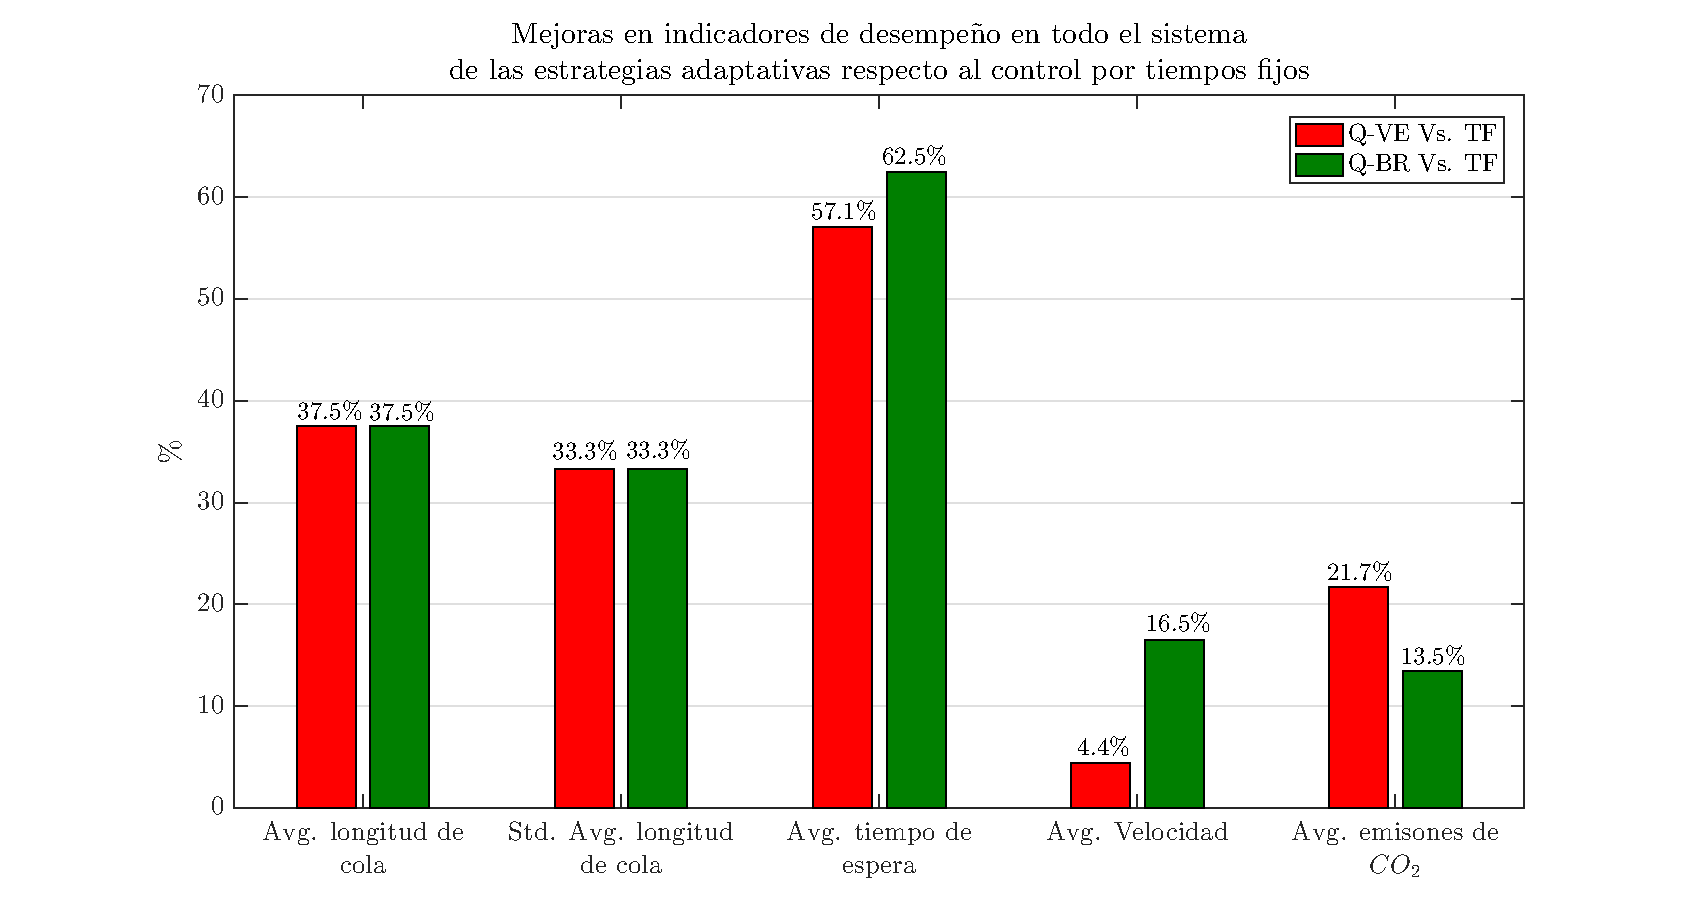
\includegraphics[scale=0.37]{./graficas/mejorasSistema2.eps}
\end{center}

\end{frame}

\subsection{Indicadores de desempeño por agente}
%----------D15: indicadores de desempeño por agente ------------------
\begin{frame}
\frametitle{Resultados}
\framesubtitle{Indicadores de desempeño por agente}
\begin{center}
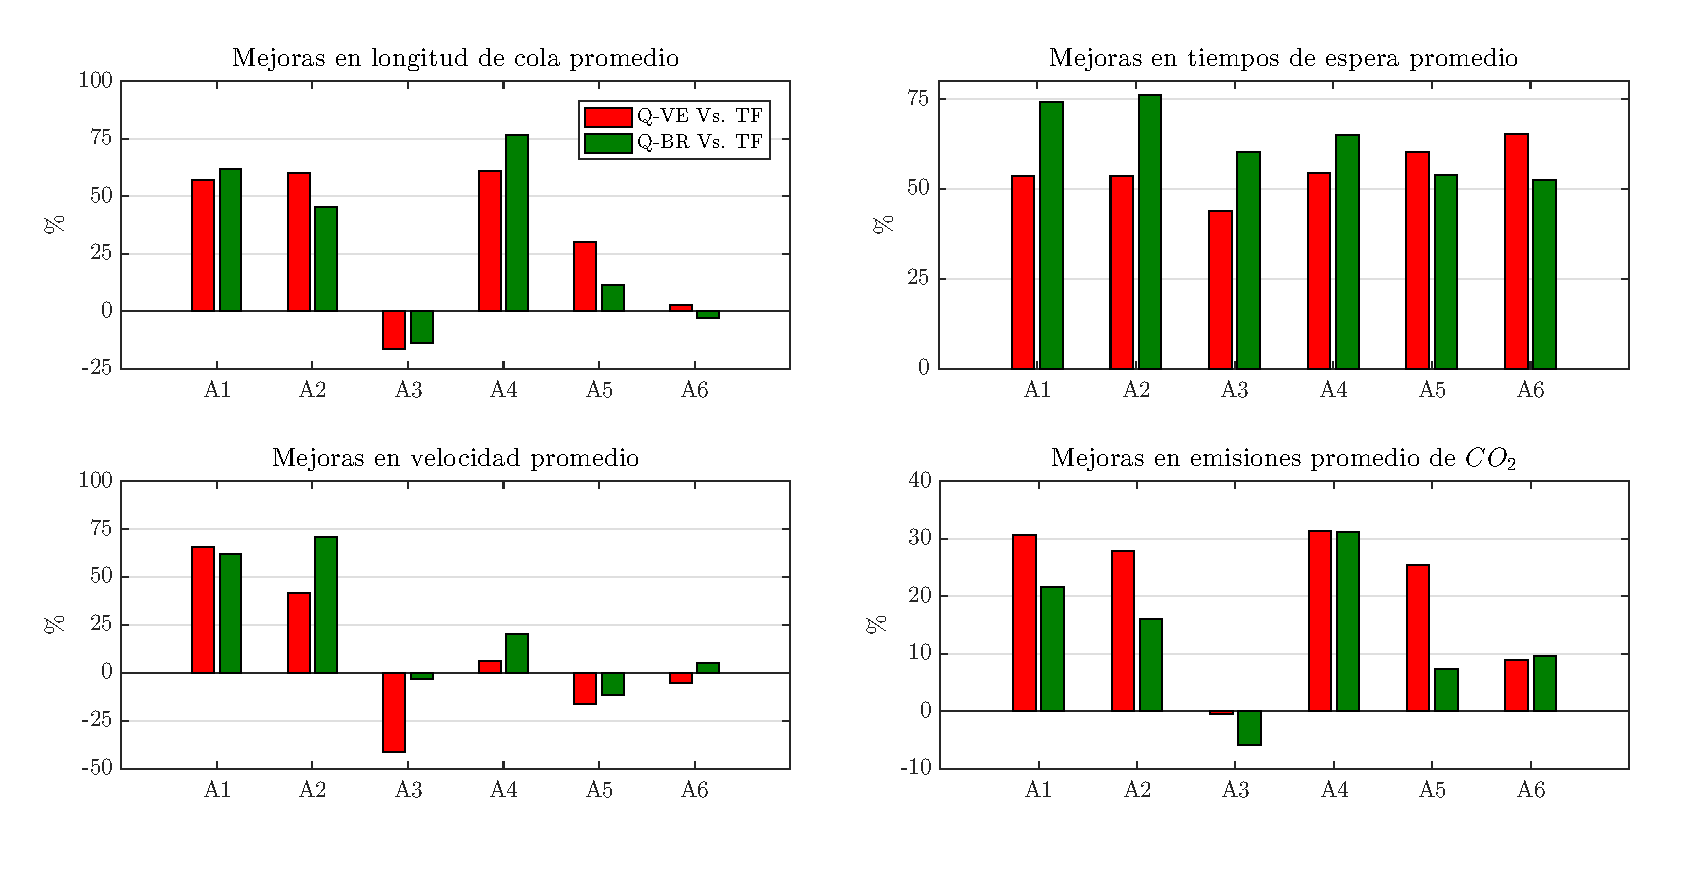
\includegraphics[scale=0.43]{./graficas/mejorasAgt.eps}
\end{center}
\end{frame}

\subsection{Tiempo de viaje}
%----------D16: tiempo de viaje ------------------
\begin{frame}
\frametitle{Resultados}
\framesubtitle{Tiempo de viaje para rutas principales}
\begin{columns}[T]

\begin{column}{.5\textwidth}
\begin{table}[]
\resizebox{0.7\textwidth}{!}{
\begin{tabular}{ccccc}
\multicolumn{1}{l}{} & \multicolumn{4}{l}{\textit{Tiempo de viaje promedio (min)}} \\
\multicolumn{1}{l}{} & Ruta 1 & Ruta 2 & Ruta 3 & \multicolumn{1}{l}{Ruta 4} \\ \hline \hline
\multicolumn{1}{c|}{TF} & 2.21 & 3.98 & 1.62 & 5.37 \\ \hline
\multicolumn{1}{c|}{Q-VE} & 1.67 & 2.09 & 1.39 & 2.85 \\ \hline
\multicolumn{1}{c|}{Q-BR} & 1.40 & 2.22 & 0.98 & 2.61 \\ \hline
\end{tabular}}
\end{table}
\end{column}

\begin{column}{.5\textwidth}
\begin{table}[]
\resizebox{0.9\textwidth}{!}{
\begin{tabular}{lcccc}
 & \multicolumn{4}{c}{\textit{Mejoras en el tiempo de viaje promedio}} \\
 & Ruta 1 & Ruta 2 & Ruta 3 & \multicolumn{1}{l}{Ruta 4} \\ \hline \hline
\multicolumn{1}{c|}{Q-VE Vs. TF} & $24.43\%$ & $47.49\%$ & $14.20\%$ & $46.93\%$ \\ \hline
\multicolumn{1}{c|}{Q-BR Vs. TF} & $36.65\%$ & $44.22\%$ & $39.51\%$ & $51.40\%$ \\ \hline
\end{tabular}}
\end{table}
\end{column}
\end{columns}

\begin{center}
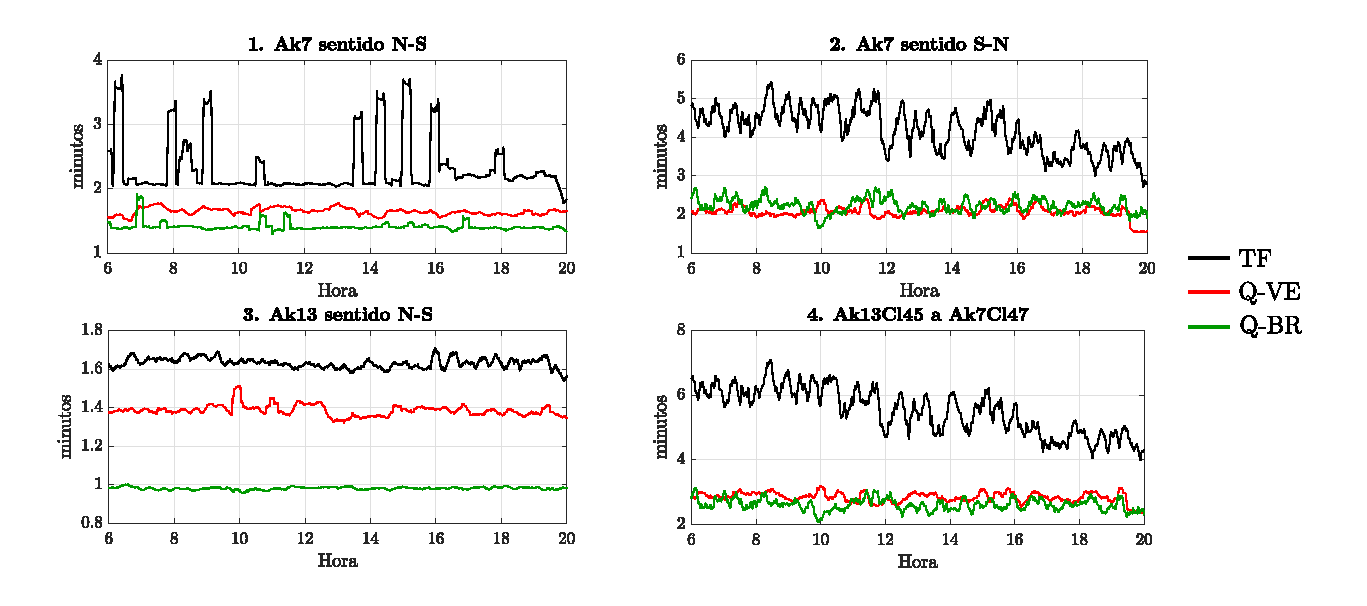
\includegraphics[scale=0.5]{./graficas/travelTime2.eps}
\end{center}
\end{frame}

\section{Conclusiones}
%----------D16: conclusiones ------------------
\begin{frame}
\frametitle{Conclusiones}
\begin{itemize}
\item Las políticas aprendidas buscan priorizar el paso contínuo de grupos de movimientos, en lugar del paso de flujos paralelos.\\
%\item Las políticas obtenidas por Q-VE y Q-BR no generan oleadas en verde, pero asignan las fases y sus duraciones con el fin de manera que se reduzca el tiempo de espera de los vehículos en el sistema, sin perjudicar la velocidad de desplazamiento.
\item Para el sistema de tránsito, la aplicación del principio de localidad en la selección de las acciones de los agentes, conlleva a una política con mejor desempeño en los objetivos de minimización.
\item El control adaptativo por medio de Q-BR presenta menor tiempo de viaje promedio y menores variaciones.
\end{itemize}

\pause

\visible<2>{
\begin{table}[]
\centering
\resizebox{\textwidth}{!}{
\begin{tabular}{@{}l|c|c@{}}
\multicolumn{1}{c|}{} & \textit{Grafos de coordinación} & \textit{Best response} \\ \hline \hline
\textcolor{blue}{Obtención de $\mathbf{a}^*$} & Exacta por medio de VE & A nivel de vecindades \\
\textcolor{blue}{Escalabilidad} & No facilmente & Completamente \\
\textcolor{blue}{Comunicaciones entre agentes} & Sujetas a cambios & Definidas \textit{a priori} \\
\textcolor{blue}{Observabilidad del sistema} & Menor & Mayor \\ \hline
\end{tabular}}
\end{table}}
\end{frame}

\section{Trabajo futuro}
%----------D16: trabajo futuro ------------------
\begin{frame}
\frametitle{Trabajo futuro}
\begin{enumerate}
\item Tener en cuenta otros objetivos en la función de recompensa (ej. velocidad promedio)
\medskip
\item Tratar el problema con un espacio de estados continuo
\medskip
\item Si se afronta el problema con un espacio de acciones continuo (ej. duraciones de las fases en una secuancia de fases fija), se podría incorporar el algoritmo de Consensus para la maximización de la función de recompensa
\end{enumerate}
\end{frame}

\section{Videos}
\begin{frame}[fragile]
\frametitle{Videos del control adaptativo por Q-BR}
\begin{block}{Simulaciones}
\href{run:./videos/6a7.mp4}{Hora pico 6am-7am}\\
\href{run:./videos/9a10.mp4}{Hora valle 9am-10am}\\
\href{run:./videos/12a1.mp4}{Hora pico 12m-1pm}
\end{block}
\end{frame}


\section{Preguntas}
%----------D16: preguntas ------------------
\begin{frame}
\begin{center}
\huge ¿Preguntas?
\end{center}
\end{frame}





\end{document}
